\section{Gegenkopplung und Stabilität \formelbuch{107}}
	\subsection{LTI-Grundglieder}	
		\begin{longtable}{|c|c|l|}
        	\specialrule{2pt}{0pt}{0pt}
        	{\bf Typ} & {\it Symbol} & {\it Gleichung, Dgl}\\
        	 & & {\it Sprungantwort}\\
        	 & & {\it Frequenzgang, Betrag und Argument}\\ \cline{2-3}
        	 & Strukturbild & {\it Nyquistdiagramm} -- {\it Bodediagramm}\\
        	\specialrule{2pt}{0pt}{0pt}
        	
        	
        	%P-Glied
        	P & \parbox[c][2cm]{3cm}{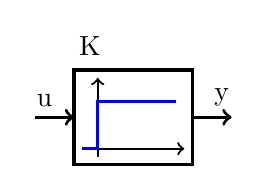
\begin{tikzpicture}
  \begin{scope}[very thick]
    \draw[->] (0,0) -- +(0.5,0) node[near start, above] {u};
    \draw (0.5,-0.6) rectangle +(1.5,1.2);
    \draw[->] (2,0) -- +(0.5,0) node[near end, above] {y};
  \end{scope}

  \node at (0.7,0.9) {K};

  % Inhalt
  \begin{scope}[shift={(0.8,-0.4)}]
    \draw[->, thick] (-0.2,0) -- +(1.3,0);
    \draw[->, thick] (0,-0.1) -- +(0,1);

    \draw[blue, very thick] (-0.2,0) -- ++(0.2,0)
       -- ++(0,0.6) -- +(1,0);
  \end{scope}

\end{tikzpicture}}
			&
			\begin{tabular}{lll}
				$y = Ku$ 		& 							& \\
				$u=1(t)$ 		& $y=K 1(t)$ 				& \\
				$G(j \omega)=K$	& $\left| G \right| = K$	& $argG=0$ \\
			\end{tabular} 
			\\ \cline{2-3}
			& \parbox[c][2cm]{3cm}{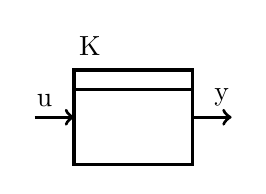
\begin{tikzpicture}
  % Box
  \begin{scope}[very thick]
    \draw[->] (0,0) -- +(0.5,0) node[near start, above] {u};
    \draw (0.5,-0.6) rectangle +(1.5,1.2);
    \draw[->] (2,0) -- +(0.5,0) node[near end, above] {y};
  \end{scope}

  % Zugemüse
  \node at (0.7,0.9) {K};
  \draw[very thick] (0.5, 0.35) -- +(1.5,0);
\end{tikzpicture}}
			& 
			\parbox[c]{3cm}{\usepgflibrary{shapes.misc}
\begin{tikzpicture}
\draw[->, thick] (-0.5,0) -- (2,0) node[below] {Re};
\draw[->, thick] (0,-0.3) -- (0,1) node[left] {Im};
\node[rounded rectangle, draw=blue, thick]  at (1,0) {};
\node at (1,0.4) {K};
\node at (0.8,-0.8) {\small{frequenzunabhängig}};
\end{tikzpicture}} \quad
			\parbox[c]{6cm}{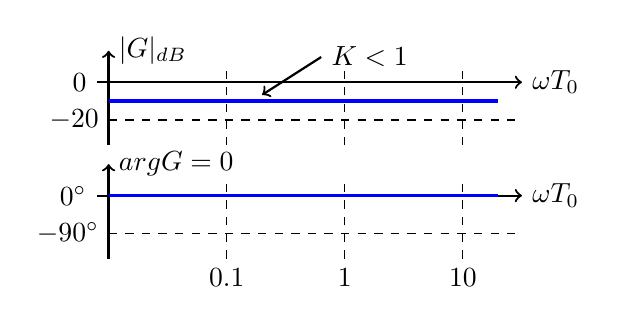
\begin{tikzpicture}[xscale=1.5, yscale=0.8]

%% Amplitude
\begin{scope}
	%% Koordinatensystem
	\draw[thick, ->] (-0.1,0) node[left] {$0$} -- (3.5,0) node[right] {$\omega T_0$};
	\draw[thick, ->] (0,-1) -- (0,0.5) node[right] {$|G|_{dB}$};
	\draw[dashed] (0,-0.6) node[left] {$-20$} -- (3.5,-0.6);
	\draw[dashed] (1,-1) -- +(0,1.2);
	\draw[dashed] (2,-1) -- +(0,1.2);
	\draw[dashed] (3,-1) -- +(0,1.2);
	%%%%%%%%%%%%%%%%

	%% Amplitudengang
	\draw[blue, very thick] (0,-0.3) -- +(3.3,0);
	\draw[<-, thick] (1.3,-0.2) -- +(0.5,0.6) node[right] {$K<1$};
\end{scope}


%% Phase
\begin{scope}[shift={(0,-1.8)}]
	%% Koordinatensystem
	\draw[thick, ->] (-0.1,0) node[left] {$0^\circ$} -- (3.5,0) node[right] {$\omega T_0$};
	\draw[thick, ->] (0,-1) -- (0,0.5) node[right] {$argG=0$};
	\draw[dashed] (0,-0.6) node[left] {$-90^\circ$} -- (3.5,-0.6);
	\draw[dashed] (1,-1) node[below] {$0.1$} -- +(0,1.2);
	\draw[dashed] (2,-1) node[below] {$1$} -- +(0,1.2);
	\draw[dashed] (3,-1) node[below] {$10$} -- +(0,1.2);
	%%%%%%%%%%%%%%%%

	%% Amplitudengang
	\draw[blue, very thick] (0,0) -- +(3.3,0);
\end{scope}

%\draw (current bounding box.south west) rectangle (current bounding box.north east);

\end{tikzpicture}}			 
	        \\
			\specialrule{2pt}{0pt}{0pt}
			
			
			%I-Glied
			I & \parbox[c][2cm]{3cm}{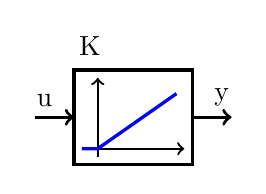
\begin{tikzpicture}
  \begin{scope}[very thick]
    \draw[->] (0,0) -- +(0.5,0) node[near start, above] {u};
    \draw (0.5,-0.6) rectangle +(1.5,1.2);
    \draw[->] (2,0) -- +(0.5,0) node[near end, above] {y};
  \end{scope}

  \node at (0.7,0.9) {K};

  % Inhalt
  \begin{scope}[shift={(0.8,-0.4)}]
    \draw[->, thick] (-0.2,0) -- +(1.3,0);
    \draw[->, thick] (0,-0.1) -- +(0,1);

    \draw[blue, very thick] (-0.2,0) -- ++(0.2,0) -- +(1,0.7);
  \end{scope}

\end{tikzpicture}}
			&
			\begin{tabular}{lll}
				$\dot{y} = Ku$ 					& 										& \\
				$u=1(t)$ 						& $y=K t$ 								& \\
				$G(j \omega)=\frac{K}{j\omega}$ & $\left| G \right| = \frac{K}{\omega}$ & $argG=-\frac{\pi}{2}$ \\
			\end{tabular}
			\\ \cline{2-3}
			& \parbox[c][2cm]{3cm}{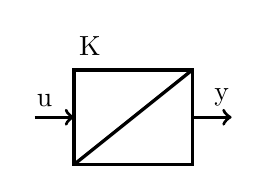
\begin{tikzpicture}
  % Box
  \begin{scope}[very thick]
    \draw[->] (0,0) -- +(0.5,0) node[near start, above] {u};
    \draw (0.5,-0.6) rectangle +(1.5,1.2);
    \draw[->] (2,0) -- +(0.5,0) node[near end, above] {y};
  \end{scope}

  % Zugemüse
  \node at (0.7,0.9) {K};
  \draw[very thick] (0.5, -0.6) -- +(1.5,1.2);
\end{tikzpicture}}
			&
			\parbox[c]{3cm}{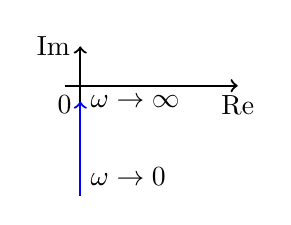
\begin{tikzpicture}
\draw[->, thick] (-0.2,0) node[below] {0} -- (2,0) node[below] {Re};
\draw[->, thick] (0,-1) -- (0,0.5) node[left] {Im};

\draw[->, blue, thick] (0,-1.4) node[above right, black] {$\omega \rightarrow 0$} 
	-- (0,-0.2) node[right, black] {$\omega \rightarrow \infty$};
%\draw (current bounding box.south west) rectangle (current bounding box.north east);
\end{tikzpicture}}
			\parbox[c]{6cm}{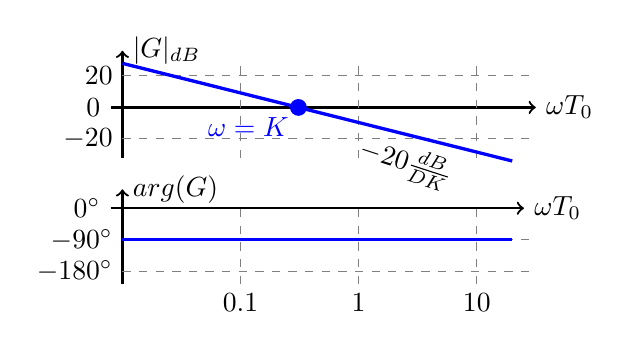
\begin{tikzpicture}[xscale=1.5, yscale=0.8]
	%% Amplitude
\begin{scope}
	%% Koordinatensystem
	\draw[thick, ->] (0,-1.2) -- (0,0.5) node[right] {$|G|_{dB}$};
	\draw[thick, ->] (-0.1,-0.4) node[left] {$0$} -- +(3.6,0) node[right] {$\omega T_0$};
	\draw[dashed,gray] (0,-0.9) node[left, black] {$-20$} -- +(3.5,0);
	\draw[dashed,gray] (0,0.1) node[left, black] {$20$} -- +(3.5,0);
	\draw[dashed,gray] (1,-1.2) -- +(0,1.5);
	\draw[dashed,gray] (2,-1.2) -- +(0,1.5);
	\draw[dashed,gray] (3,-1.2) -- +(0,1.5);
	%%%%%%%%%%%%%%%%

	%% Amplitudengang
	\draw[blue, very thick] (0,0.3) -- +(3.3,-1.55) node[near end, below, rotate=-18, black] {$-20\frac{dB}{DK}$};
	\draw(1.49,-0.4) node[draw,circle,inner sep=2pt,fill, blue] {};
	\node at (1.49, -0.4) [anchor = north east, blue] {$\omega = K$};
	
\end{scope}


%% Phase
\begin{scope}[shift={(0,-2.2)}]
	%% Koordinatensystem
	\draw[thick, ->] (-0.1,0.2) node[left] {$0^\circ$} -- +(3.5,0) node[right] {$\omega T_0$};
	\draw[thick, ->] (0,-1) -- (0,0.5) node[right] {$arg(G)$};
	\draw[dashed,gray] (0,-0.3) node[left, black] {$-90^\circ$} -- +(3.5,0);
	\draw[dashed,gray] (0,-0.8) node[left, black] {$-180^\circ$} -- +(3.5,0);
	\draw[dashed, gray] (1,-1) node[below, black] {$0.1$} -- +(0,1.2);
	\draw[dashed,gray] (2,-1) node[below, black] {$1$} -- +(0,1.2);
	\draw[dashed,gray] (3,-1) node[below, black] {$10$} -- +(0,1.2);
	%%%%%%%%%%%%%%%%

	%% Amplitudengang
	\draw[blue, very thick] (0,-0.3) -- +(3.3,0);
\end{scope}

%\draw (current bounding box.south west) rectangle (current bounding box.north east);
\end{tikzpicture}} 
	        \\
			\specialrule{2pt}{0pt}{0pt}
			
			
			%D-Glied
			D & \parbox[c][2cm]{3cm}{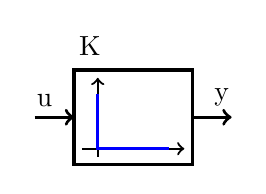
\begin{tikzpicture}
  \begin{scope}[very thick]
    \draw[->] (0,0) -- +(0.5,0) node[near start, above] {u};
    \draw (0.5,-0.6) rectangle +(1.5,1.2);
    \draw[->] (2,0) -- +(0.5,0) node[near end, above] {y};
  \end{scope}

  \node at (0.7,0.9) {K};

  % Inhalt
  \begin{scope}[shift={(0.8,-0.4)}]
    \draw[->, thick] (-0.2,0) -- +(1.3,0);
    \draw[->, thick] (0,-0.1) -- +(0,1);

    \draw[blue, very thick] (0,0.7) -- ++(0,-0.7) -- +(0.9,0);
  \end{scope}

\end{tikzpicture}}
			&
			\begin{tabular}{lll}
				$y = K\dot{u}$					&										& \\
				$u=1(t)$						& $y=K \delta (t)$						& \\
				$G(j \omega)=K j\omega$			& $\left| G \right| = K\omega$			& $argG=\frac{\pi}{2}$
			\end{tabular}
			\\ \cline{2-3}
			& \parbox[c][2cm]{3cm}{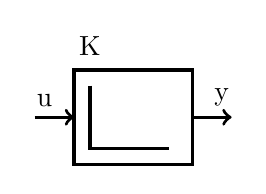
\begin{tikzpicture}
  % Box
  \begin{scope}[very thick]
    \draw[->] (0,0) -- +(0.5,0) node[near start, above] {u};
    \draw (0.5,-0.6) rectangle +(1.5,1.2);
    \draw[->] (2,0) -- +(0.5,0) node[near end, above] {y};
  \end{scope}

  % Zugemüse
  \node at (0.7,0.9) {K};
  \draw[very thick] (0.7, 0.4) -- ++(0,-0.8) -- ++(1,0);
\end{tikzpicture}}			
			&
			\parbox[c]{3cm}{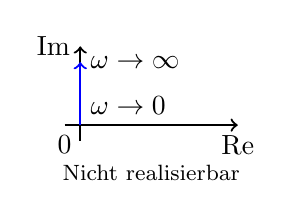
\begin{tikzpicture}
\draw[->, thick] (-0.2,0) node[below] {0} -- (2,0) node[below] {Re};
\draw[->, thick] (0,-0.2) -- (0,1) node[left] {Im};

\draw[->, blue, thick] (0,0) node[above right, black] {$\omega \rightarrow 0$} 
	-- (0,0.8) node[right, black] {$\omega \rightarrow \infty$};
\draw[] (0.9,-0.6) node {\footnotesize{Nicht realisierbar}};
%\draw (current bounding box.south west) rectangle (current bounding box.north east);
\end{tikzpicture}}
			\parbox[c]{6cm}{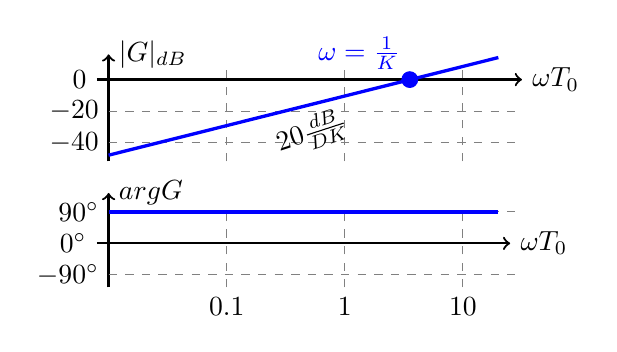
\begin{tikzpicture}[xscale=1.5, yscale=0.8]
	%% Amplitude
\begin{scope}
	%% Koordinatensystem
	\draw[thick, ->] (0,-1.2) -- (0,0.5) node[right] {$|G|_{dB}$};
	\draw[thick, ->] (-0.1,0.1) node[left] {$0$} -- +(3.6,0) node[right] {$\omega T_0$};
	\draw[dashed,gray] (0,-0.9) node[left, black] {$-40$} -- +(3.5,0);
	\draw[dashed,gray] (0,-0.4) node[left, black] {$-20$} -- +(3.5,0);
	\draw[dashed,gray] (1,-1.2) -- +(0,1.5);
	\draw[dashed,gray] (2,-1.2) -- +(0,1.5);
	\draw[dashed,gray] (3,-1.2) -- +(0,1.5);
	%%%%%%%%%%%%%%%%

	%% Amplitudengang
	\draw[blue, very thick] (0,-1.1) -- +(3.3,1.55) node[midway, below, rotate=18, black] {$20\frac{dB}{DK}$};
	\draw(2.55,0.1) node[draw,circle,inner sep=2pt,fill, blue] {};
	\node at (2.55, 0.1) [anchor = south east, blue] {$\omega = \frac{1}{K}$};
\end{scope}


%% Phase
\begin{scope}[shift={(0,-2.2)}]
	%% Koordinatensystem
	\draw[thick, ->] (-0.1,-0.3) node[left] {$0^\circ$} -- +(3.5,0) node[right] {$\omega T_0$};
	\draw[thick, ->] (0,-1) -- (0,0.5) node[right] {$argG$};
	\draw[dashed,gray] (0,0.2) node[left, black] {$90^\circ$} -- +(3.5,0);
	\draw[dashed,gray] (0,-0.8) node[left, black] {$-90^\circ$} -- +(3.5,0);
	\draw[dashed, gray] (1,-1) node[below, black] {$0.1$} -- +(0,1.2);
	\draw[dashed,gray] (2,-1) node[below, black] {$1$} -- +(0,1.2);
	\draw[dashed,gray] (3,-1) node[below, black] {$10$} -- +(0,1.2);
	%%%%%%%%%%%%%%%%

	%% Amplitudengang
	\draw[blue, very thick] (0,0.2) -- +(3.3,0);
\end{scope}

%\draw (current bounding box.south west) rectangle (current bounding box.north east);
\end{tikzpicture}} 
	        \\
			\specialrule{2pt}{0pt}{0pt}
			
			
			%PT1_Glied
			$PT_1$ & \parbox[c][2cm]{3cm}{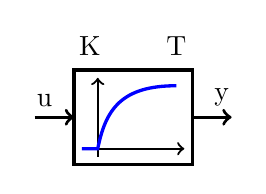
\begin{tikzpicture}
  \begin{scope}[very thick]
    \draw[->] (0,0) -- +(0.5,0) node[near start, above] {u};
    \draw (0.5,-0.6) rectangle +(1.5,1.2);
    \draw[->] (2,0) -- +(0.5,0) node[near end, above] {y};
  \end{scope}

  \node at (0.7,0.9) {K};
  \node at (1.8,0.9) {T};

  % Inhalt
  \begin{scope}[shift={(0.8,-0.4)}]
    \draw[->, thick] (-0.2,0) -- +(1.3,0);
    \draw[->, thick] (0,-0.1) -- +(0,1);

    \draw[blue, very thick] (-0.2,0) -- ++(0.2,0)
              .. controls (0.1,0.5) and (0.3,0.8) .. (1,0.8);
  \end{scope}

\end{tikzpicture}}
			&
			\begin{tabular}{lll}
				$T\dot{y}+y=Ku$							& $y(0)=0$									& \\
				$u=1(t)$								& $y=K \left[ 1-e^{- \frac{t}{T}}\right]$	& \\
				$G(j \omega)= \frac{K}{1+j\omega T}$	& $\left| G \right| = \frac{K}{\sqrt{1+(\omega T)^2}}$ &
				$argG=-\arctan(\omega T)$
			\end{tabular}
			\\ \cline{2-3}
			& \parbox[c][2cm]{3cm}{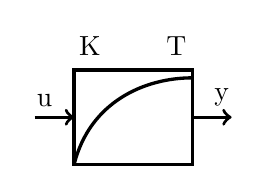
\begin{tikzpicture}
  \begin{scope}[very thick]
    \draw[->] (0,0) -- +(0.5,0) node[near start, above] {u};
    \draw (0.5,-0.6) rectangle +(1.5,1.2);
    \draw[->] (2,0) -- +(0.5,0) node[near end, above] {y};
  \end{scope}

 % Zugemüse
 \node at (0.7,0.9) {K};
 \node at (1.8,0.9) {T};
 \draw[very thick] (0.5,-0.6)  .. controls (0.7,0.2) and (1.4,0.5) .. (2,0.5);

\end{tikzpicture}}	
			&
			\parbox[c]{3.7cm}{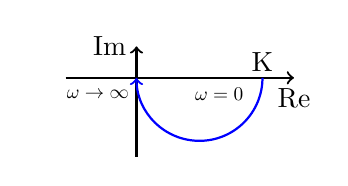
\begin{tikzpicture}
\draw[->, thick] (-0.9,0) -- (2,0) node[below] {Re};
\draw[->, thick] (0,-1) -- (0,0.4) node[left] {Im};

\node at (1.6,0.2) {K};
\draw[blue, thick, ->] (1.6,0) arc (0:-180:0.8);

\scalebox{0.7}{
  \node at (-0.7,-0.3) {$\omega \rightarrow \infty$};
  \node at (1.5, -0.3) {$\omega = 0$};
}
\end{tikzpicture}}
			\parbox[c]{6cm}{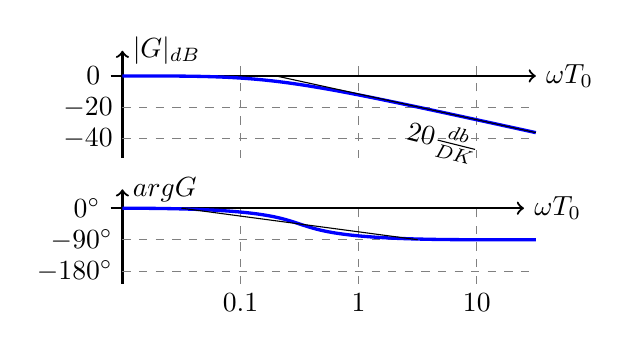
\begin{tikzpicture}[xscale=1.5, yscale=0.8]
	%% Amplitude
\begin{scope}
	%% Koordinatensystem
	\draw[thick, ->] (0,-1.2) -- (0,0.5) node[right] {$|G|_{dB}$};
	\draw[dashed,gray] (1,-1.2) -- +(0,1.5);
	\draw[dashed,gray] (2,-1.2) -- +(0,1.5);
	\draw[dashed,gray] (3,-1.2) -- +(0,1.5);
	
	\draw[thick, ->] (-0.1,0.1) node[left] {$0$} -- +(3.6,0) node[right] {$\omega T_0$};
	\draw[dashed,gray] (0,-0.9) node[left, black] {$-40$} -- +(3.5,0);
	\draw[dashed,gray] (0,-0.4) node[left, black] {$-20$} -- +(3.5,0);

	%%%%%%%%%%%%%%%%

	%% Amplitudengang
	\draw[blue, very thick] (0,0.1) .. controls (1.3,0.1) .. (3.5,-0.8) 
			node[very near end, below, rotate=-14, color=black] {$20 \frac{db}{DK}$};
	\draw (1.3,0.1) -- (3.5, -0.8);
\end{scope}


%% Phase
\begin{scope}[shift={(0,-2.2)}]
	%% Koordinatensystem
	\draw[thick, ->] (0,-1) -- (0,0.5) node[right] {$argG$};
	\draw[dashed, gray] (1,-1) node[below, black] {$0.1$} -- +(0,1.2);
	\draw[dashed,gray] (2,-1) node[below, black] {$1$} -- +(0,1.2);
	\draw[dashed,gray] (3,-1) node[below, black] {$10$} -- +(0,1.2);
	
	\draw[thick, ->] (-0.1,0.2) node[left] {$0^\circ$} -- +(3.5,0) node[right] {$\omega T_0$};
	\draw[dashed,gray] (0,-0.3) node[left, black] {$-90^\circ$} -- +(3.5,0);
	\draw[dashed,gray] (0,-0.8) node[left, black] {$-180^\circ$} -- +(3.5,0);

	%%%%%%%%%%%%%%%%

	%% Amplitudengang
	\draw[blue, very thick] (0,0.2) .. controls (2.2,0.2) and (0.8,-0.3) .. (3,-0.3) -- +(0.5,0);
	\draw (0.5,0.2) -- (2.5,-0.3);
	
\end{scope}

%\draw (current bounding box.south west) rectangle (current bounding box.north east);
\end{tikzpicture}}
	        \\
			\specialrule{2pt}{0pt}{0pt}
			
			
			%PT2_Glied
			$PT_2$ &
			\begin{minipage}{3cm}
	        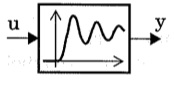
\includegraphics[width=3cm]{./images/PT2_glied.jpg}
	        \end{minipage}
	        &
	        \begin{tabular}{lll}
	        	$T^2\ddot{y}+2\zeta T \dot{y}+y=Ku$ & $\ddot{y}+2\zeta\omega_n \dot{y}+\omega_n^2y=K\omega_n^2u$ & \\
	        	$y(0)=0$ & $\dot{y}(0)=0$ & $\omega_n=\frac{1}{T}$ \\
	        	\multicolumn{3}{l}{
	        		$y=K \left[1-\frac{1}{\sqrt{1-\zeta^2}}e^{-\zeta\omega_n t}\sin
               		\left( \sqrt{1-\zeta^2} \omega_n t+arcos(\zeta) \right)\right]$
               	} \\
               	$G(j \omega)= \frac{K}{(j \omega T)^2 + 2 \zeta T (j\omega) + 1}$ & $\left| G \right| = \frac{K}{\sqrt{\left[1+(j\omega
               	T)^2\right]^2+\left[2\zeta \omega T \right]^2}}$ & \\
               	$\arg G=-\arctan  \frac{2\zeta \omega T}{(j\omega T)^2+1}$ & $0 \leq\omega T \leq 1$ & \\
               	$\arg G=\arctan \frac{2\zeta \omega T}{(j \omega T)^2+1}-\pi$ & $1 \leq\omega T \leq \infty$ & \\
	        	
	        \end{tabular}
			\\ \cline{2-3}
			& \begin{minipage}{3cm}
	        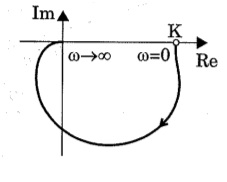
\includegraphics[angle = {-0.3}, width=3cm]{./images/PT2_Nyq.jpg}
	        \end{minipage}
			& \begin{minipage}{12cm}
	        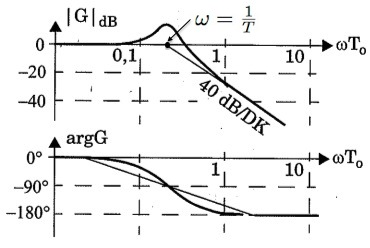
\includegraphics[angle = {0.2}, width=8cm]{./images/PT2_Bode.jpg}
	        \end{minipage} \rule[-5mm]{0mm}{35mm}
	        \\
			\specialrule{2pt}{0pt}{0pt}
			
			
			%Tt_Glied
			$T_t$ &
	        \parbox[c][2cm]{3cm}{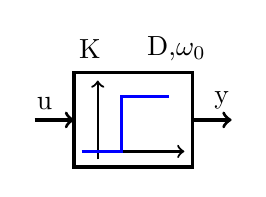
\begin{tikzpicture}
  \begin{scope}[very thick]
    \draw[->] (0,0) -- +(0.5,0) node[near start, above] {u};
    \draw (0.5,-0.6) rectangle +(1.5,1.2);
    \draw[->] (2,0) -- +(0.5,0) node[near end, above] {y};
  \end{scope}

  \node at (0.7,0.9) {K};
  \node at (1.8,0.9) {D,$\omega_0$};

  % Inhalt
  \begin{scope}[shift={(0.8,-0.4)}]
    \draw[->, thick] (-0.2,0) -- +(1.3,0);
    \draw[->, thick] (0,-0.1) -- +(0,1);

    \draw[blue, very thick] (-0.2,0) -- ++(0.5,0) -- ++(0,0.7) -- +(0.6,0);
  \end{scope}

\end{tikzpicture}}
	        &
	        \begin{tabular}{lll}
	        	$y=\begin{cases}
  					0 & 0<t<T_t \\
  					u(t-T_t) & t \geq T_t
					\end{cases}$ & & \\
				$u=1(t)$ & $y=1(t-T_t)$ & \\
				$G(j \omega)= e^{-j\omega T_t}$ & $\left| G \right| = 1$ & $argG=-\omega T_t$
	        \end{tabular}
			\\ \cline{2-3}
			& \parbox[c][2cm]{3cm}{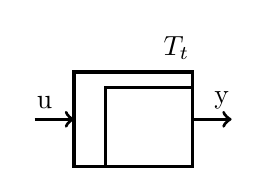
\begin{tikzpicture}
  \begin{scope}[very thick]
    \draw[->] (0,0) -- +(0.5,0) node[near start, above] {u};
    \draw (0.5,-0.6) rectangle +(1.5,1.2);
    \draw[->] (2,0) -- +(0.5,0) node[near end, above] {y};
  \end{scope}

% Zugemüse
\node at (1.8,0.9) {$T_t$};

\draw[very thick] (0.9,-0.6) -- ++(0,1) -- +(1.1,0);
\end{tikzpicture}}
			& 
			\parbox[c]{3cm}{\usetikzlibrary{decorations.markings}
\begin{tikzpicture}
\useasboundingbox (-1.4,-1.4) rectangle (1.9,1.4);
\draw[->, thick] (-1.1,0) -- (1.6,0) node[above] {Re};
\draw[->, thick] (0,-1) -- (0,1.1) node[left] {Im};

\draw (0.8,0.05) arc(90:450:0.05) node[above right] {\small{1}};
\draw (-0.8,0.05) arc(90:450:0.05) node[above left] {\small{-1}};

\draw[blue, thick,
	decoration={
		markings,
		mark= at position 0.9 with {\arrow{<}}
	},
	postaction={decorate}
] (0.8,0) arc (0:360:0.8);

\scalebox{0.7}{
  \node at (1.3,-1.5) {$2\pi$-periodisch};
  \node at (1.6, -0.3) {$\omega = 0$};
}
%\draw (current bounding box.south west) rectangle (current bounding box.north east);
\end{tikzpicture}}
			\parbox[c]{6cm}{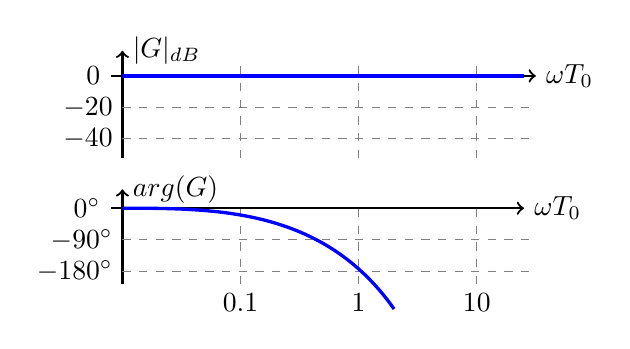
\begin{tikzpicture}[xscale=1.5, yscale=0.8]
	%% Amplitude
\begin{scope}
	%% Koordinatensystem
	\draw[thick, ->] (0,-1.2) -- (0,0.5) node[right] {$|G|_{dB}$};
	\draw[dashed,gray] (1,-1.2) -- +(0,1.5);
	\draw[dashed,gray] (2,-1.2) -- +(0,1.5);
	\draw[dashed,gray] (3,-1.2) -- +(0,1.5);
	
	\draw[thick, ->] (-0.1,0.1) node[left] {$0$} -- +(3.6,0) node[right] {$\omega T_0$};
	\draw[dashed,gray] (0,-0.9) node[left, black] {$-40$} -- +(3.5,0);
	\draw[dashed,gray] (0,-0.4) node[left, black] {$-20$} -- +(3.5,0);

	%%%%%%%%%%%%%%%%

	%% Amplitudengang
	\draw[blue, very thick] (0,0.1) -- +(3.4,0);
\end{scope}


%% Phase
\begin{scope}[shift={(0,-2.2)}]
	%% Koordinatensystem
	\draw[thick, ->] (0,-1) -- (0,0.5) node[right] {$arg(G)$};
	\draw[dashed, gray] (1,-1) node[below, black] {$0.1$} -- +(0,1.2);
	\draw[dashed,gray] (2,-1) node[below, black] {$1$} -- +(0,1.2);
	\draw[dashed,gray] (3,-1) node[below, black] {$10$} -- +(0,1.2);
	
	\draw[thick, ->] (-0.1,0.2) node[left] {$0^\circ$} -- +(3.5,0) node[right] {$\omega T_0$};
	\draw[dashed,gray] (0,-0.3) node[left, black] {$-90^\circ$} -- +(3.5,0);
	\draw[dashed,gray] (0,-0.8) node[left, black] {$-180^\circ$} -- +(3.5,0);

	%%%%%%%%%%%%%%%%

	%% Amplitudengang
	\draw[blue, very thick] (0,0.2) .. controls (0.8,0.2) and (1.7,0.2) .. (2.3,-1.4);	
\end{scope}

%\draw (current bounding box.south west) rectangle (current bounding box.north east);
\end{tikzpicture}}
	        \\
			\specialrule{2pt}{0pt}{0pt}
        \end{longtable}

%----------------------------------------------------------------------------------------
%
%	Tabelle aus Buch Seite 124
%
%
%	\subsection{Der Frequenzgang \formelbuch{117}}
%		\begin{tabular}{| c | c | c | c |}
%		    \hline
%	        $P$-Glied & $I$-Glied & $PT_1$-Glied & $T_t$-Glied \\
%	        \begin{minipage}{3cm}
%	        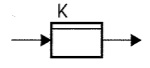
\includegraphics[width=3cm]{./images/pglied}
%	        \end{minipage} &
%			\begin{minipage}{3cm}
%	        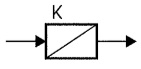
\includegraphics[width=3cm]{./images/iglied}
%	        \end{minipage} &
%			\begin{minipage}{4cm}
%	        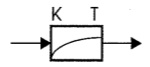
\includegraphics[width=3cm]{./images/pt1glied}
%	        \end{minipage} &
%			\begin{minipage}{3cm}
%	        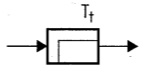
\includegraphics[width=3cm]{./images/tglied}
%	        \end{minipage} \\
%	        \hline
%	        $y=Ku$ & $\dot{y} = Ku$ & $T\dot{y}+y = Ku$ & $y=u(t-T_t)$ \\
%	        &  &  & $t\geq T_t$ \\
%	        \hline
%	        $G(j\omega)=K$ & $G(j\omega)= \frac{K}{j\omega}$ &
%	        $G(j\omega)=\frac{K}{1+j\omega T}$ &
%	        $G(j\omega)=e^{-j\omega T_t}$\\
%	        & & & \\
%	        \hline
%	        $\left| G \right| = K$ & $\left| G \right| = \frac{K}{\omega}$ &
%	        $\left| G \right| = \frac{K}{\sqrt{1+(|\omega T)^2}}$ &
%	        $\left| G \right| = 1$ \\
%	        $argG=0$ & $argG= -\frac{\pi}{2}$ & $argG=-\arctan(\omega T)$ &
%	        $argG= - \omega T_t$\\
%	        & & &  \\
%	        \hline
%	        & & & \\
%	        \begin{minipage}{3cm}
%	        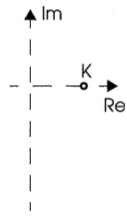
\includegraphics[width=2.7cm]{./images/fg_pglied}
%	        \end{minipage} &
%			\begin{minipage}{3cm}
%	        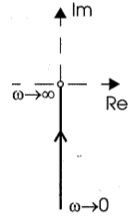
\includegraphics[width=3cm]{./images/fg_iglied}
%	        \end{minipage} &
%			\begin{minipage}{4cm}
%	        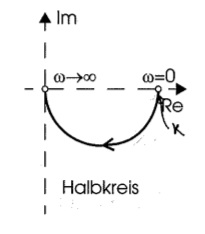
\includegraphics[width=4cm]{./images/fg_pt1glied}
%	        \end{minipage} &
%			\begin{minipage}{3cm}
%	        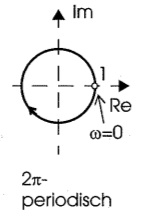
\includegraphics[width=3cm]{./images/fg_tglied}
%	        \end{minipage} \\
%			& & & \\
%	        \hline
%	        \end{tabular}

%----------------------------------------------------------------------------------------



	\subsection{Stabilitätsproblem \formelbuch{108}}
		\begin{minipage}{5cm}
		\fbox{$K_I T_t=\frac{\pi}{2}$} \\
		\fbox{$K_I=\omega_\pi$}
		\end{minipage}
		\begin{minipage}{13cm}
        $K_I$: Stabilitätsgrenze \\
        $\omega_\pi$: Phasenschnittfrequenz
        \end{minipage}


	\subsection{Nyquistkriterium \formelbuch{129}}
		Der geschlossene Regelkreis ist genau dann stabil, wenn beim Durchlauf der
		Ortskurve in Richtung zunehmender Frequenz der kritische Punkt -1 \glqq zur
		Linken\grqq\ liegt.
		
	\subsection{Phasenreserve und Verstärkungsreserve \formelbuch{132}}
		\begin{tabular}{l|ll}
			$K_RK_{Rres}=K_{R\pi}$ & $K_R$ & Reglerverstärkung ($K_R < K_{R\pi} \rightarrow$ Regelung stabil, $K_R > K_{R\pi} \rightarrow$ Regelung
			instabil	) \\
			$K_{Rres}=\frac{1}{\left| G(j\omega_{\pi})\right|}$ & $K_{Rres}$ & 	Verstärkungsreserve mit Regler (Amplitudenres., gain margin) \\
			$argG_0=-\pi+\Phi_{res}$ & $K_{R\pi}$ & kritische Verstärkung (Verstärkung ohne	Regler) \\
			$argG_0(\omega_\pi)=-\pi$ & $\omega_\pi$ & Phasenschnittfrequenz\\
			$|G_0(j\omega_D)|=1$ & $\omega_D$ & Durchtrittsfrequenz \\
			& $\Phi_{res}$ & Phasenreserve
		\end{tabular}
		
        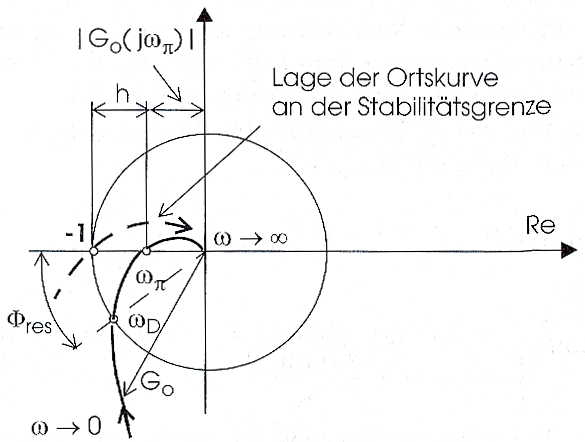
\includegraphics[width=6.2cm]{./images/phasenreserve.png}
			
	\subsection{Sprungantwort und Stabilität \formelbuch{135}}
		\subsubsection{Stabilitätssatz für ein System 2. Ordnung \formelbuch{137}}
			Ein System ist genau dann stabil, wenn {\bf alle} Koeffizienten der
			homogenen Dgl. positiv (oder alle negativ) und ungleich 0 sind.\\
			$\ddot{y}+a_1\dot{y}+a_0y=F(u)$
			
		\subsubsection{Stabilitätssatz für die Sprungantwort}
			Ein LTI-System ist genau dann stabil, wenn die Sprungantwort einem
			konstantem Wert zustrebt.